\section{Desarrollo del sistema}

\begin{frame}{Conjunto de datos}
    \centering
    \begin{tikzpicture}[
        stat/.style={
            rectangle,
            rounded corners=5pt,
            minimum width=3.25cm,
            minimum height=1.6cm,
            align=center,
            font=\small,
            draw=black!25
        },
        detalle/.style={
            rectangle,
            rounded corners=5pt,
            fill=black!5,
            draw=black!20,
            text width=9.5cm,
            minimum height=0.82cm,
            align=center,
            font=\small
        }
    ]
        \node[stat, fill=blue!12, draw=blue!35] (sujetos) {
            {\Large\bfseries 24}\\
            participantes
        };
        \node[stat, fill=green!14, draw=green!35!black, right=0.55cm of sujetos] (emociones) {
            {\Large\bfseries 3}\\
            emociones
        };
        \node[stat, fill=orange!18, draw=orange!45, right=0.55cm of emociones] (archivos) {
            {\Large\bfseries 72}\\
            archivos crudos
        };

        \node[detalle, below=0.65cm of emociones] (d1) {\textbf{JOY}, \textbf{NEUTRO} y \textbf{SAD}: una grabación por participante y emoción};
        \node[detalle, below=0.28cm of d1] (d2) {Los archivos se conservan en formato EDF antes de aplicar preprocesado o limpieza.};
    \end{tikzpicture}
\end{frame}

\begin{frame}{Flujo general del sistema}
    \centering
    \resizebox{!}{0.76\textheight}{
    \begin{tikzpicture}[
        node distance=0.8cm,
        fase/.style={
            rectangle,
            rounded corners=3pt,
            minimum width=4.1cm,
            minimum height=0.78cm,
            align=center,
            font=\bfseries\small,
            draw=black!45
        },
        fasepeq/.style={
            rectangle,
            rounded corners=3pt,
            minimum width=3.55cm,
            minimum height=0.58cm,
            align=center,
            font=\bfseries\scriptsize,
            draw=black!45
        },
        dato/.style={
            align=center,
            font=\scriptsize,
            text width=3.2cm,
            fill=white,
            inner sep=1pt
        },
        flecha/.style={-{Latex[length=2.5mm]}, thick, draw=black!55}
    ]
        \node[fase, fill=blue!18] (prep) {Preprocesado};

        \node[fasepeq, fill=blue!18, below=of prep] (comprobacion) {Control de sujetos válidos};

        \node[fase, fill=green!18, below=of comprobacion] (features) {Extracción de características};

        \node[fase, fill=violet!18, below left=0.9cm and 0.3cm of features] (sep) {Separabilidad};

        \node[fase, fill=yellow!22, below right=0.9cm and 0.3cm of features] (train) {Entrenamiento y evaluación};

        \node[fase, fill=orange!22, below=of train] (explain) {Explicabilidad};

        \node[dato, above=0.3cm of prep] (raw) {registros EDF};
        \node[dato, below=0.3cm of sep] (sepout) {resultados de separabilidad};
        \node[dato, below=0.3cm of explain] (expout) {resultados de explicabilidad};

        \draw[flecha] (raw) -- (prep);
        \draw[flecha] (prep) -- (comprobacion)
            node[midway, right, dato] {épocas preprocesadas};
        \draw[flecha] (comprobacion) -- (features)
            node[midway, right, dato] {épocas preprocesadas\\y sujetos aptos};
        \draw[flecha] (features) -- (sep)
            node[midway, left, dato] {características};
        \draw[flecha] (features) -- (train)
            node[midway, right, dato] {características};
        \draw[flecha] (sep) -- (sepout);
        \draw[flecha] (train) -- (explain)
            node[midway, right, dato] {modelos \textit{within}\\y características};
        \draw[flecha] (explain) -- (expout);
    \end{tikzpicture}
    }
\end{frame}

\begin{frame}{Preprocesado}
    \centering
    \begin{tikzpicture}[
        bloque/.style={
            rectangle,
            rounded corners=4pt,
            minimum width=3.8cm,
            minimum height=0.82cm,
            align=center,
            font=\small\bfseries,
            draw=black!45,
            text width=3.55cm
        },
        detalle/.style={
            font=\scriptsize,
            align=center,
            text width=3.55cm
        },
        flecha/.style={-{Latex[length=2.2mm]}, thick, draw=black!55}
    ]
        \node[bloque, fill=blue!14] (filtro) at (0,0)
            {Filtrado y preparación};
        \node[detalle, below=0.04cm of filtro] (filtrod)
            {canales, montaje, ruido eléctrico y remuestreo};

        \node[bloque, fill=orange!16] (artefactos) at (4.25,0)
            {Limpieza de artefactos};
        \node[detalle, below=0.04cm of artefactos] (artefactosd)
            {canales problemáticos, referencia, ICA e interpolación};

        \node[bloque, fill=green!16] (epocas) at (8.5,0)
            {Segmentación en épocas};
        \node[detalle, below=0.04cm of epocas] (epocasd)
            {ventanas con información emocional útil};

        \draw[flecha] (filtro.east) -- (artefactos.west);
        \draw[flecha] (artefactos.east) -- (epocas.west);
    \end{tikzpicture}

    \vspace{0.18cm}
    \begin{columns}[T,onlytextwidth]
        \begin{column}{0.49\textwidth}
            \centering
            {\scriptsize\bfseries EDF crudo con marcas temporales}\\[-0.5mm]
            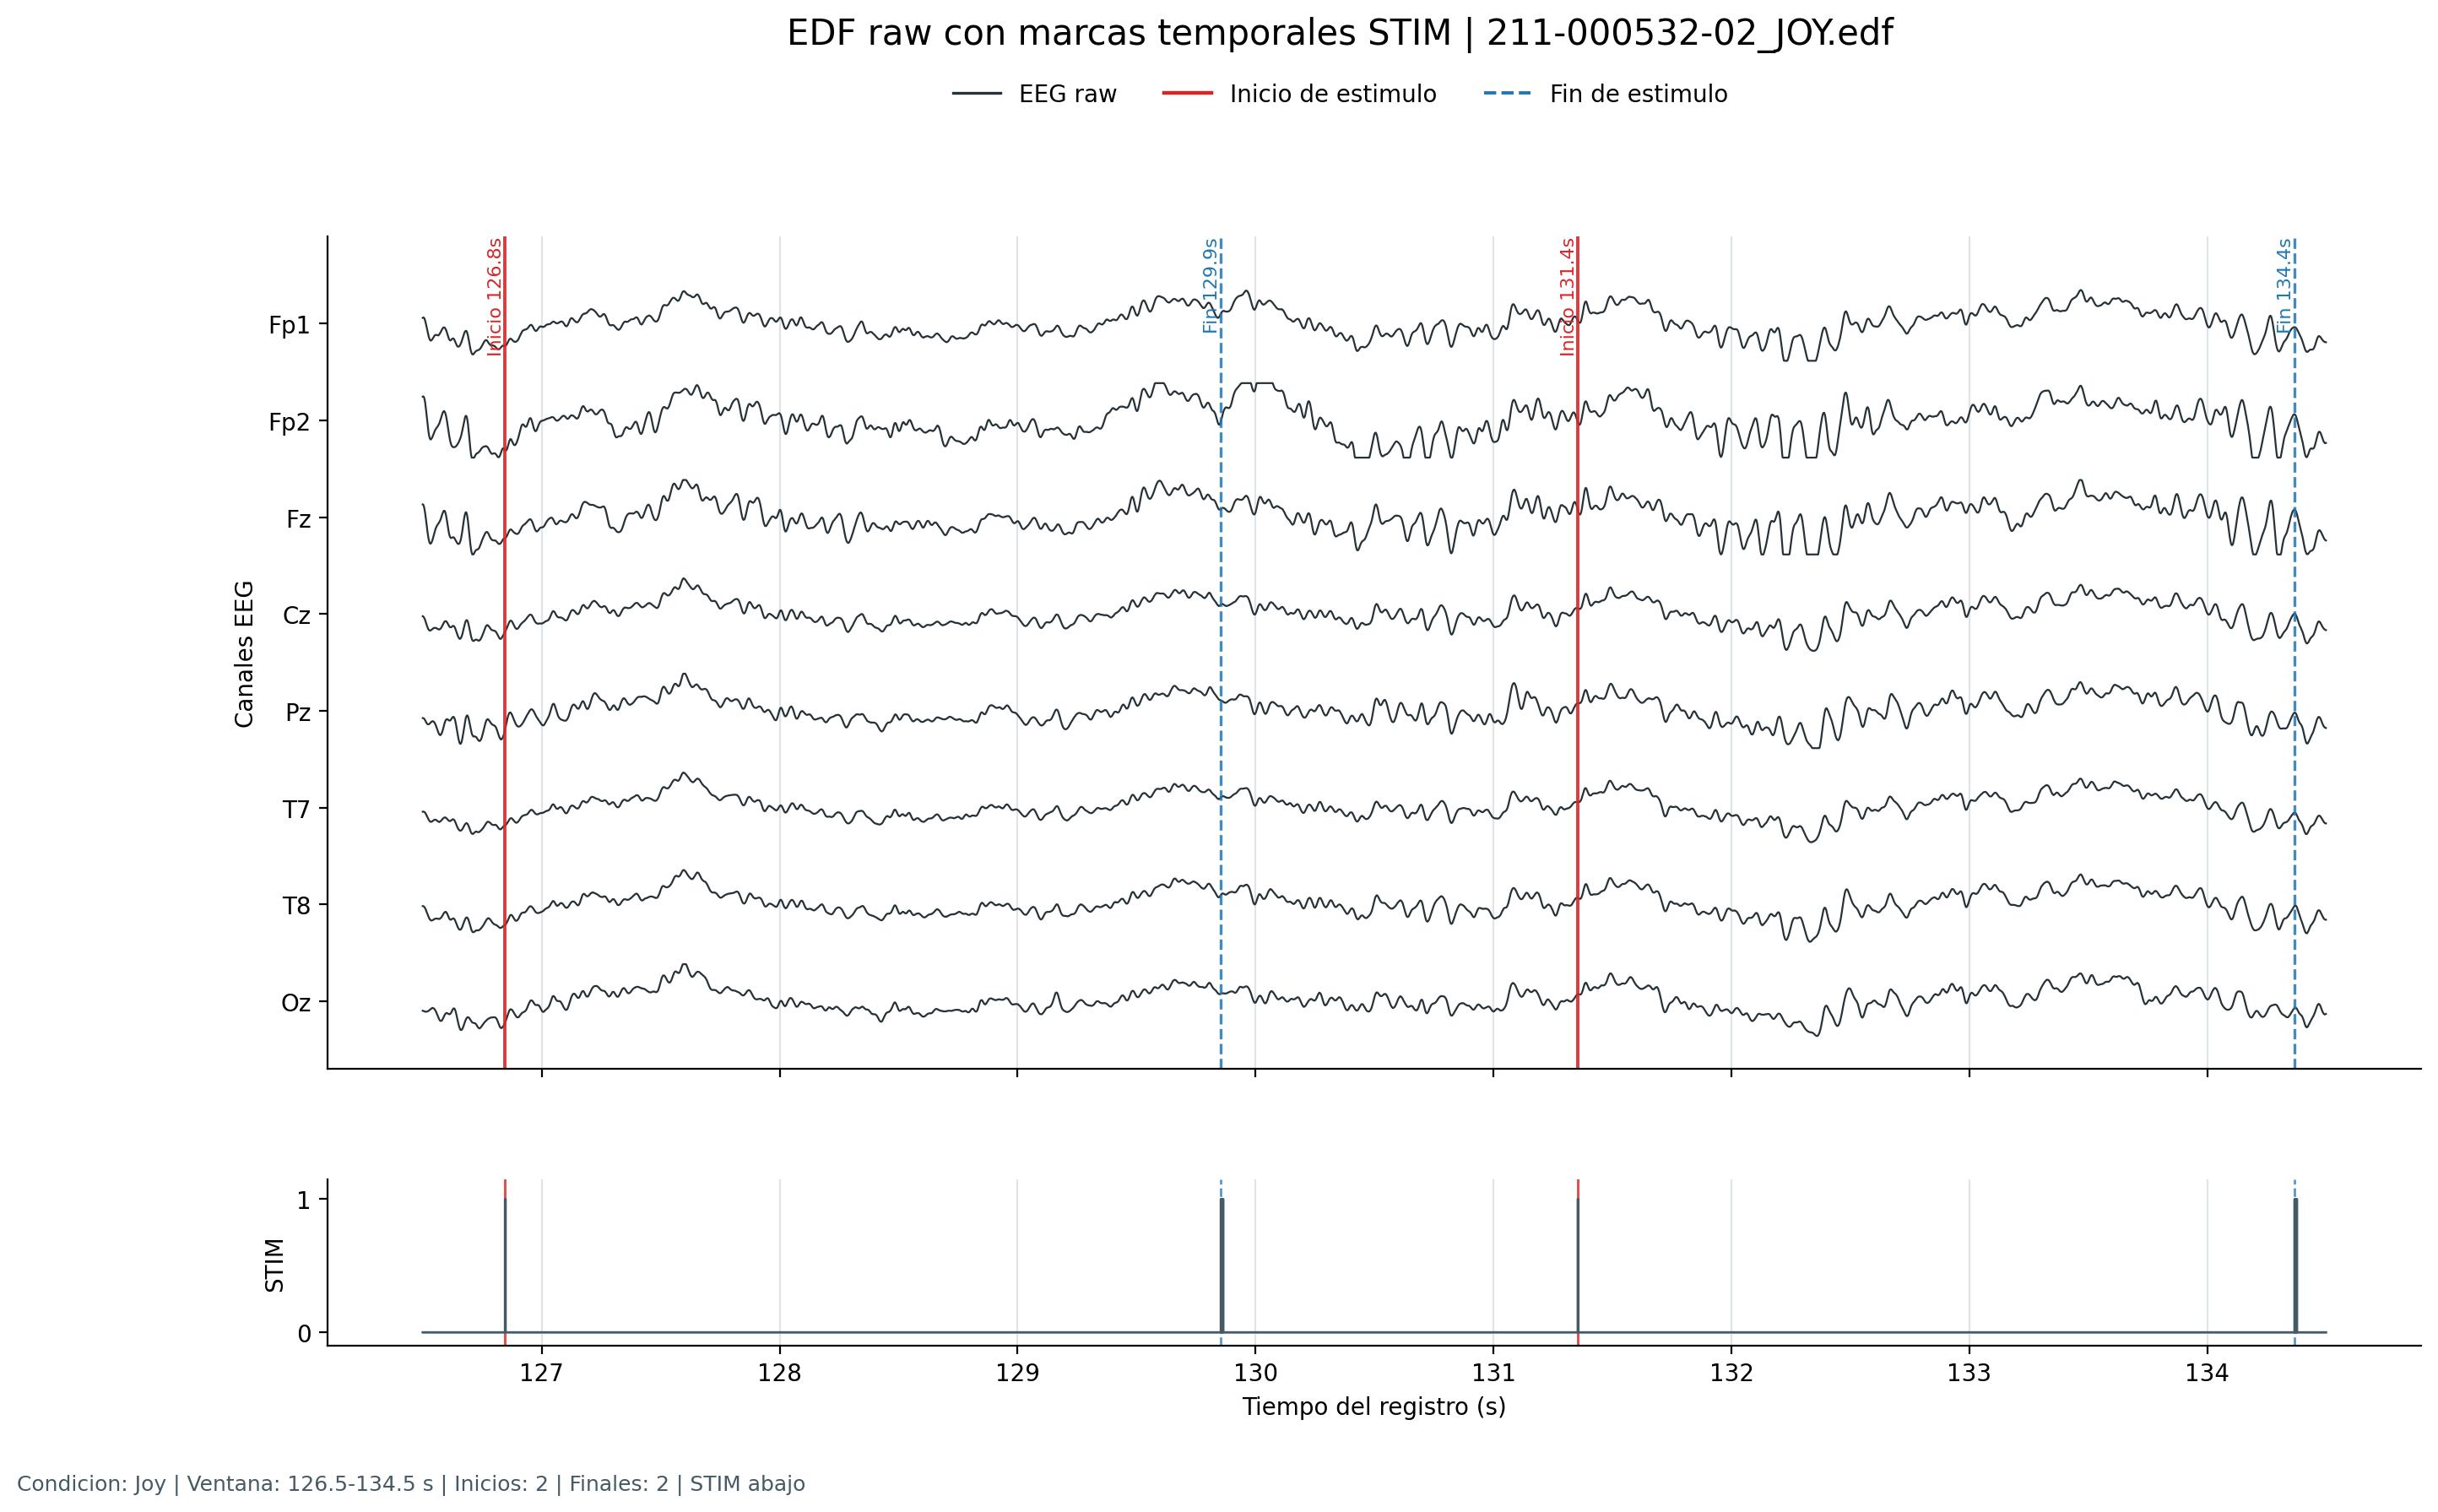
\includegraphics[width=\textwidth]{figs/edf_raw_marcas_temporales.png}
        \end{column}

        \begin{column}{0.49\textwidth}
            \centering
            {\scriptsize\bfseries Épocas preprocesadas consecutivas}\\[-0.5mm]
            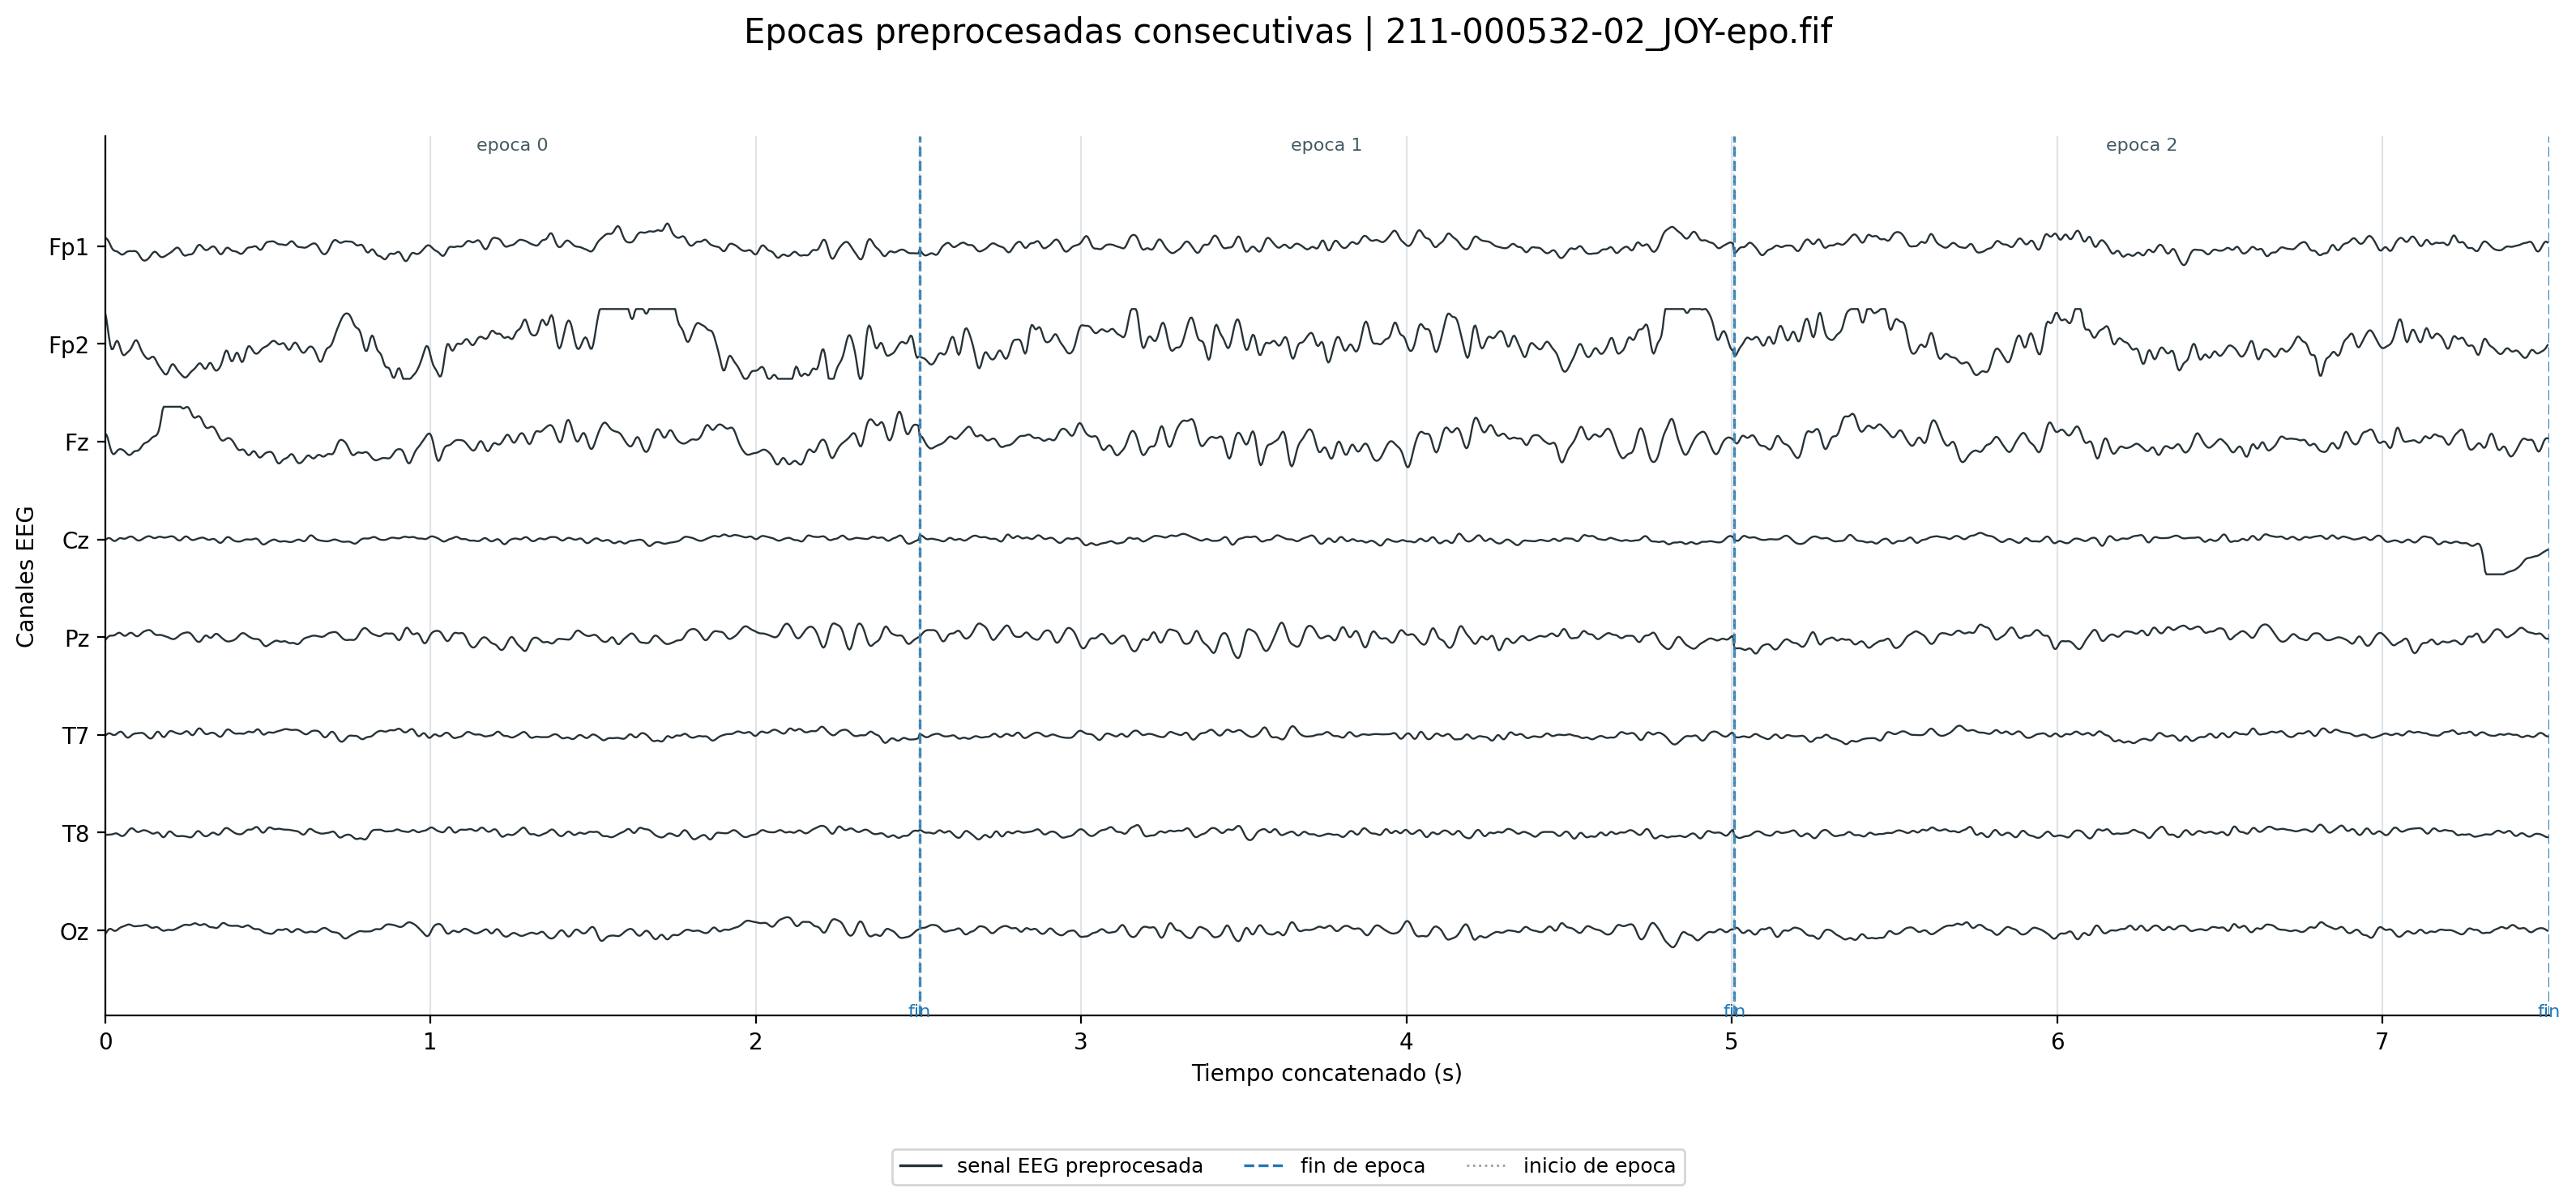
\includegraphics[width=\textwidth]{figs/epocas_consecutivas_marcas.png}
        \end{column}
    \end{columns}
\end{frame}

\begin{frame}{Control de sujetos válidos}
    \centering
    \begin{tikzpicture}[
        card/.style={
            rectangle,
            rounded corners=5pt,
            text width=9.7cm,
            minimum height=1.0cm,
            align=left,
            font=\small,
            inner xsep=10pt,
            draw=black!25
        },
        num/.style={
            circle,
            minimum size=0.58cm,
            font=\bfseries\small,
            text=white,
            fill=urjcred
        }
    ]
        \node[card, fill=blue!10] (a) {
            \hspace{0.55cm}\textbf{Completitud}\\
            \hspace{0.55cm}El sujeto debe tener épocas para JOY, NEUTRO y SAD.
        };
        \node[num, left=0.18cm of a.west] {1};

        \node[card, fill=green!10, below=0.35cm of a] (b) {
            \hspace{0.55cm}\textbf{Balance de épocas}\\
            \hspace{0.55cm}Se revisa que una emoción no quede muy por debajo del resto.
        };
        \node[num, left=0.18cm of b.west] {2};

        \node[card, fill=orange!13, below=0.35cm of b] (c) {
            \hspace{0.55cm}\textbf{Revisión espectral}\\
            \hspace{0.55cm}Se comprueba que la señal conserve una forma espectral compatible con EEG.
        };
        \node[num, left=0.18cm of c.west] {3};

        \node[
            rectangle,
            rounded corners=4pt,
            fill=urjcred!8,
            draw=urjcred!35,
            text width=8.2cm,
            align=center,
            font=\small,
            below=0.45cm of c
        ] {Salida: lista de sujetos aptos para extracción de características.};
    \end{tikzpicture}
\end{frame}

\begin{frame}{Extracción de características}
    \begin{columns}[c,onlytextwidth]
        \begin{column}{0.38\textwidth}
            \centering
            \begin{tikzpicture}[
                bloque/.style={
                    rectangle,
                    rounded corners=4pt,
                    minimum width=4.15cm,
                    minimum height=0.86cm,
                    align=center,
                    font=\small\bfseries,
                    draw=black!45,
                    text width=3.75cm
                },
                detalle/.style={
                    font=\scriptsize,
                    align=center,
                    text width=3.85cm
                },
                flecha/.style={-{Latex[length=2.2mm]}, thick, draw=black!55}
            ]
                \node[bloque, fill=green!14] (epocas) {Épocas limpias};
                \node[detalle, below=0.03cm of epocas] (epocasd)
                    {FIF + sujetos válidos};

                \node[bloque, fill=blue!12, below=0.52cm of epocasd] (psd)
                    {PSD y promedio};
                \node[detalle, below=0.03cm of psd] (psdd)
                    {Welch + media dentro de cada banda};

                \node[bloque, fill=orange!14, below=0.52cm of psdd] (features)
                    {Features finales};
                \node[detalle, below=0.03cm of features]
                    {canal + banda + asimetría};

                \draw[flecha] (epocasd) -- (psd);
                \draw[flecha] (psdd) -- (features);
            \end{tikzpicture}
        \end{column}

        \begin{column}{0.59\textwidth}
            \centering
            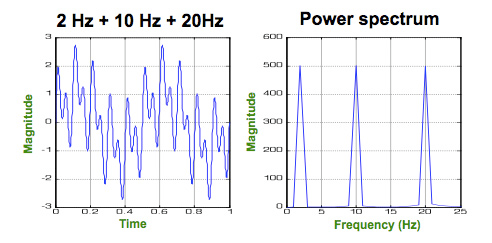
\includegraphics[width=0.82\textwidth]{../memoria/figs/psd.png}

            \vspace{0.20cm}
            \renewcommand{\arraystretch}{1.08}
            {\scriptsize
            \setlength{\tabcolsep}{4pt}
            \begin{tabular}{@{}llc@{}}
                \toprule
                \multicolumn{3}{c}{\textbf{Dataset de entrada al modelo}} \\
                \midrule
                Filas & épocas EEG & 2754 \\
                Columnas & características & 150 \\
                \midrule
                \multicolumn{3}{c}{\textbf{Bloques de características}} \\
                \midrule
                Alpha/Beta & canal + banda, ej. \texttt{FC4\_Beta} & 124 \\
                Asim. Alpha & der.-izq., ej. \texttt{F4-F3} & 26 \\
                \bottomrule
            \end{tabular}
            }

            \vspace{0.18cm}
            {\scriptsize Asimetría: ayuda al modelo a captar diferencias izquierda-derecha.}
        \end{column}
    \end{columns}
\end{frame}

\begin{frame}{Selección de bandas}
    \centering
    \begin{tikzpicture}[
        banda/.style={
            rectangle,
            rounded corners=5pt,
            minimum width=5.25cm,
            minimum height=2.05cm,
            align=center,
            draw=black!35,
            text width=4.75cm,
            inner sep=8pt
        },
        motivo/.style={
            rectangle,
            rounded corners=4pt,
            minimum width=9.8cm,
            minimum height=0.62cm,
            align=center,
            draw=black!25,
            font=\small,
            text width=9.25cm,
            inner sep=5pt
        },
        flecha/.style={-{Latex[length=2.2mm]}, thick, draw=black!55}
    ]
        \node[banda, fill=yellow!20] (alpha) {
            {\Large\bfseries Alpha}\\[1mm]
            {\normalsize 8--12 Hz}\\[2mm]
            {\small estado despierto, tranquilo\\y actividad de referencia}
        };

        \node[banda, fill=green!18, right=0.65cm of alpha] (beta) {
            {\Large\bfseries Beta}\\[1mm]
            {\normalsize 12--30 Hz}\\[2mm]
            {\small atención, procesamiento activo\\y respuesta al estímulo}
        };

        \coordinate (centro) at ($(alpha.south)!0.5!(beta.south)$);

        \node[motivo, fill=urjcred!8, below=0.64cm of centro] (decision) {
            Escucha pasiva: sujeto despierto, ojos cerrados y audio emocional.
        };

        \node[motivo, fill=gray!10, below=0.20cm of decision] {
            Delta, Theta y Gamma quedan fuera del modelo final.
        };

        \coordinate (decisionL) at ([xshift=-2.45cm]decision.north);
        \coordinate (decisionR) at ([xshift=2.45cm]decision.north);
        \draw[flecha] (alpha.south) -- (decisionL);
        \draw[flecha] (beta.south) -- (decisionR);
    \end{tikzpicture}
\end{frame}

\begin{frame}{Entrenamiento y evaluación}
    \centering
    \resizebox{0.98\textwidth}{!}{
    \begin{tikzpicture}[
        carril/.style={
            rounded corners=10pt,
            draw=black!12,
            line width=0.6pt
        },
        etiqueta/.style={
            rectangle,
            rounded corners=6pt,
            minimum width=2.7cm,
            minimum height=0.82cm,
            align=center,
            font=\small\bfseries,
            draw=black!25,
            text width=2.35cm,
            inner sep=5pt
        },
        pasoent/.style={
            rectangle,
            rounded corners=6pt,
            minimum width=2.55cm,
            minimum height=0.78cm,
            align=center,
            font=\scriptsize,
            draw=black!25,
            text width=2.25cm,
            inner sep=5pt
        },
        entrenamiento/.style={
            rectangle,
            rounded corners=8pt,
            minimum width=2.75cm,
            minimum height=1.05cm,
            align=center,
            font=\small,
            draw=black!30,
            fill=yellow!18
        },
        flecha/.style={-{Latex[length=2.2mm]}, thick, draw=black!55}
    ]
        \path[carril, fill=orange!6] (-6.9,0.55) rectangle (1.65,1.85);
        \path[carril, fill=green!6]  (-6.9,-1.35) rectangle (1.65,-0.05);

        \node[etiqueta, fill=orange!18] (general) at (-5.65,1.20) {
            Modelo general
        };

        \node[pasoent, fill=white] (generalcv) at (-2.85,1.20) {
            Stratified\\GroupKFold\\
            por sujeto
        };

        \node[pasoent, fill=white] (generalnorm) at (0.05,1.20) {
            Referencia NEUTRO\\
            sujetos de train
        };

        \node[etiqueta, fill=green!15] (intra) at (-5.65,-0.70) {
            Modelo\\
            por sujeto
        };

        \node[pasoent, fill=white] (intracv) at (-2.85,-0.70) {
            5 \textit{folds}\\temporales
        };

        \node[pasoent, fill=white] (intranorm) at (0.05,-0.70) {
            Referencia NEUTRO\\
            train del sujeto
        };

        \node[entrenamiento] (train) at (3.35,0.25) {
            Entrenamiento\\[-0.6mm]
            {\scriptsize dentro de cada \textit{fold}}
        };

        \node[entrenamiento, fill=urjcred!8] (eval) at (6.45,0.25) {
            Evaluación\\[-0.6mm]
            {\scriptsize métricas y matriz}
        };

        \draw[flecha] (general) -- (generalcv);
        \draw[flecha] (generalcv) -- (generalnorm);
        \draw[flecha] (intra) -- (intracv);
        \draw[flecha] (intracv) -- (intranorm);
        \draw[flecha] (generalnorm.east) -- ++(0.55,0) |- (train.west);
        \draw[flecha] (intranorm.east) -- ++(0.55,0) |- (train.west);
        \draw[flecha] (train) -- (eval);
    \end{tikzpicture}
    }
\end{frame}

\begin{frame}{Explicabilidad}
    \centering
    \resizebox{0.98\textwidth}{!}{
    \begin{tikzpicture}[
        paso/.style={
            rectangle,
            rounded corners=7pt,
            minimum width=2.55cm,
            minimum height=1.05cm,
            align=center,
            font=\small,
            draw=black!30,
            text width=2.25cm,
            inner sep=6pt
        },
        nota/.style={
            rectangle,
            rounded corners=7pt,
            minimum width=8.2cm,
            minimum height=0.65cm,
            align=center,
            font=\scriptsize,
            draw=black!20,
            fill=orange!8
        },
        flecha/.style={-{Latex[length=2mm]}, thick, draw=black!55}
    ]
        \node[paso, fill=green!12] (sujeto) at (-5.3,0.55) {
            Modelo\\por sujeto
        };

        \node[paso, fill=green!8] (folds) at (-2.6,0.55) {
            5 \textit{folds}\\
        };

        \node[paso, fill=yellow!14] (logreg) at (0.1,0.55) {
            Regresión\\logística
        };

        \node[paso, fill=orange!14] (shap) at (2.8,0.55) {
            SHAP\\sobre test
        };

        \node[paso, fill=orange!20] (topomaps) at (5.5,0.55) {
            Topomaps\\de importancia
        };

        \node[nota] at (0.1,-1.15) {
            SHAP no muestra la señal EEG directa: muestra qué canales y bandas influyen más en la decisión del modelo.
        };

        \draw[flecha] (sujeto) -- (folds);
        \draw[flecha] (folds) -- (logreg);
        \draw[flecha] (logreg) -- (shap);
        \draw[flecha] (shap) -- (topomaps);
    \end{tikzpicture}
    }
\end{frame}
